\section{Neural Search and Reasoning Optimisation}

\begin{frame}{}
    \LARGE Advanced Reasoning: \textbf{Neural Search and Reasoning Optimisation}

    \vspace{1em}
    \normalsize Can search be written into the token stream and learned, and can it then be made cheap?
\end{frame}

\begin{frame}{Search as a Sequence: Stream of Search and Meta-CoT}
    \begin{itemize}\itemsep0.35em
        \item \textbf{Stream of Search.} Take a symbolic search on the Countdown game and \emph{write it out as text}: states, expansions, dead ends, backtracking. Train a transformer on those streams, including the failed ones.
        \begin{itemize}\itemsep0.1em
            \item 51.3\% of held-out problems solved. Training on optimal solutions only: 25.7\%.
            \item After further self-improvement it solves problems that none of the symbolic strategies solved.
        \end{itemize}
        \item \textbf{Meta-CoT} turns this into a thesis about reasoning data. Textbook solutions show the steps $\mathbf{s}_1,\dots,\mathbf{s}_n$. They never show the search $\mathbf{z}_1,\dots,\mathbf{z}_K$ that found them:
        \[
            p(\mathbf a,\mathbf s_{1:n}\mid\mathbf q)\;\propto\;\int p(\mathbf a,\mathbf s_{1:n}\mid\mathbf z_{1:K},\mathbf q)\,\prod_{t=1}^{K}p(\mathbf z_t\mid\mathbf z_{<t},\mathbf q)\;d\mathbf Z
        \]
        \item \textbf{The proposed recipe:} generate search traces with MCTS or A*, verify outcomes, linearise them, fine-tune on them, then use RL to make the search efficient.
    \end{itemize}
    \vspace{0.05em}
    \src{Gandhi et al., ``Stream of Search,'' \href{https://arxiv.org/abs/2404.03683}{arXiv:2404.03683}. Xiang et al., ``Towards System 2 Reasoning in LLMs: Learning How to Think With Meta Chain-of-Thought,'' \href{https://arxiv.org/abs/2501.04682}{arXiv:2501.04682}.}
\end{frame}

\begin{frame}{Does RL Create Search Ability, or Sharpen It?}
    \begin{itemize}\itemsep0.45em
        \item The optimistic view: with thought and answer sampled together, a model ``can learn a search algorithm''. R1 and rStar-Math show verification and backtracking nobody programmed.
        \item \textbf{A sobering measurement.} Compare an RL-trained model with its base model at pass@$k$:
    \end{itemize}
    \begin{center}
    \small
    \begin{adjustbox}{max width=\linewidth}\begin{tabular}{lcc}
        \toprule
        & \textbf{Small $k$} & \textbf{Large $k$} \\
        \midrule
        RL-trained model & \textbf{wins} & \\
        Base model & & \textbf{reaches higher coverage} \\
        \bottomrule
    \end{tabular}\end{adjustbox}
    \end{center}
    \begin{itemize}\itemsep0.45em
        \item Six RL algorithms behave alike. Distillation, by contrast, \emph{can} add new reasoning patterns.
        \item \textbf{A 2026 formulation:} a base model with $N_{\text{Base}}$ samples matches an RL model with $N_{\text{RL}}$ samples when $N_{\text{Base}}\approx\alpha\,N_{\text{RL}}^{\beta}$. On this reading, much of the RL gain is \emph{sampling efficiency}.
    \end{itemize}
    \vspace{0.1em}
    \src{Welleck, CMU 11-711 (Nov 2025). Yue et al., ``Does Reinforcement Learning Really Incentivize Reasoning Capacity in LLMs Beyond the Base Model?'' NeurIPS 2025, \href{https://arxiv.org/abs/2504.13837}{arXiv:2504.13837}. Sun et al., ``A Budgeted Search Perspective,'' \href{https://arxiv.org/abs/2609.01274}{arXiv:2609.01274} (abstract only).}
\end{frame}

\begin{frame}{To Backtrack or Not to Backtrack}
    \begin{itemize}\itemsep0.4em
        \item A controlled test of the idea. Train one model to search with backtracking, on depth-first traces. Train another to answer directly, and give it parallel best-of-$n$. \textbf{Match the FLOPs.}
    \end{itemize}
    \begin{center}
    \small
    \renewcommand{\arraystretch}{1.15}
    \begin{adjustbox}{max width=\linewidth}\begin{tabular}{>{\raggedright\arraybackslash}p{2.6cm}>{\raggedright\arraybackslash}p{4.6cm}>{\raggedright\arraybackslash}p{6.2cm}}
        \toprule
        \textbf{Task} & \textbf{Winner at equal compute} & \textbf{Why} \\
        \midrule
        Countdown & \textbf{direct answers in parallel}, at every budget & the backtracking model copies a \emph{prescribed} search order, and spends tokens being verbose \\
        Sudoku & \textbf{backtracking} & the problem needs deep search \\
        \bottomrule
    \end{tabular}\end{adjustbox}
    \end{center}
    \begin{itemize}\itemsep0.4em
        \item \textbf{Then add RL.} The backtracking model discovers new strategies: about 70\%, against 57\% for the search it imitated. The direct model \emph{loses} its edge under parallel sampling.
    \end{itemize}
    \vspace{0.1em}
    \takeaway{Imitating a \emph{fixed} search algorithm can lose to cheap parallel sampling. It pays when the task needs depth, or when RL loosens the imitation.}
    \src{Qin et al. (Harvard), ``To Backtrack or Not to Backtrack: When Sequential Search Limits Model Reasoning,'' \href{https://arxiv.org/abs/2504.07052}{arXiv:2504.07052}.}
\end{frame}

\begin{frame}{Compressing the Search: Searchformer and Dualformer}
    \centering
    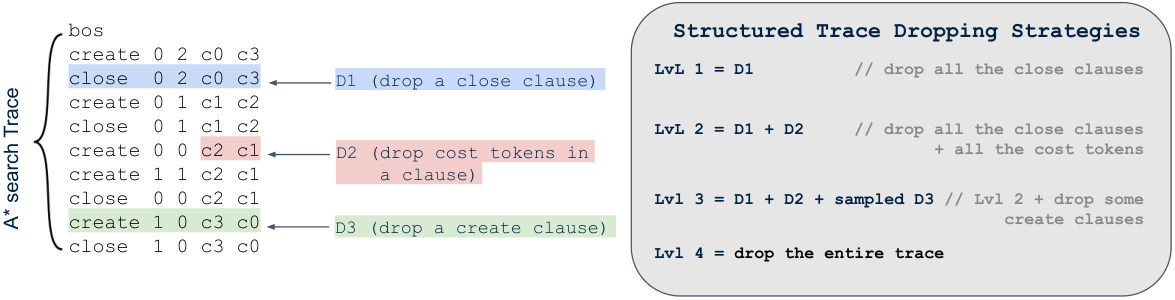
\includegraphics[width=0.92\linewidth,height=0.33\textheight,keepaspectratio]{images/advanced-reasoning/dualformer_trace.png}
    \begin{itemize}\itemsep0.3em
        \item \textbf{Searchformer.} Serialise every A* operation as tokens. Then bootstrap: sample, keep the \emph{shorter} traces that still give an optimal plan, fine-tune, repeat. Sokoban: 93.7\% solved optimally, with up to 26.8\% fewer search steps than A* itself.
        \item \textbf{Dualformer.} Drop parts of the trace at random during training (figure). One model then has a \textbf{fast}, a \textbf{slow} and an \textbf{auto} mode. Mazes, slow mode: 97.6\% optimal against 93.3\%, with 45.5\% fewer steps.
        \item Trace length as a controllable mode: a small-scale ancestor of today's effort dials.
    \end{itemize}
    \src{Lehnert et al. (Meta FAIR), ``Beyond A*: Better Planning with Transformers via Search Dynamics Bootstrapping,'' \href{https://arxiv.org/abs/2402.14083}{arXiv:2402.14083}. Su et al. (Meta), ``Dualformer: Controllable Fast and Slow Thinking,'' \href{https://arxiv.org/abs/2410.09918}{arXiv:2410.09918}.}
\end{frame}

\begin{frame}{Width Inside the Model, and Cheaper Depth}
    \begin{columns}[T,onlytextwidth]
        \column{0.47\textwidth}
        \centering
        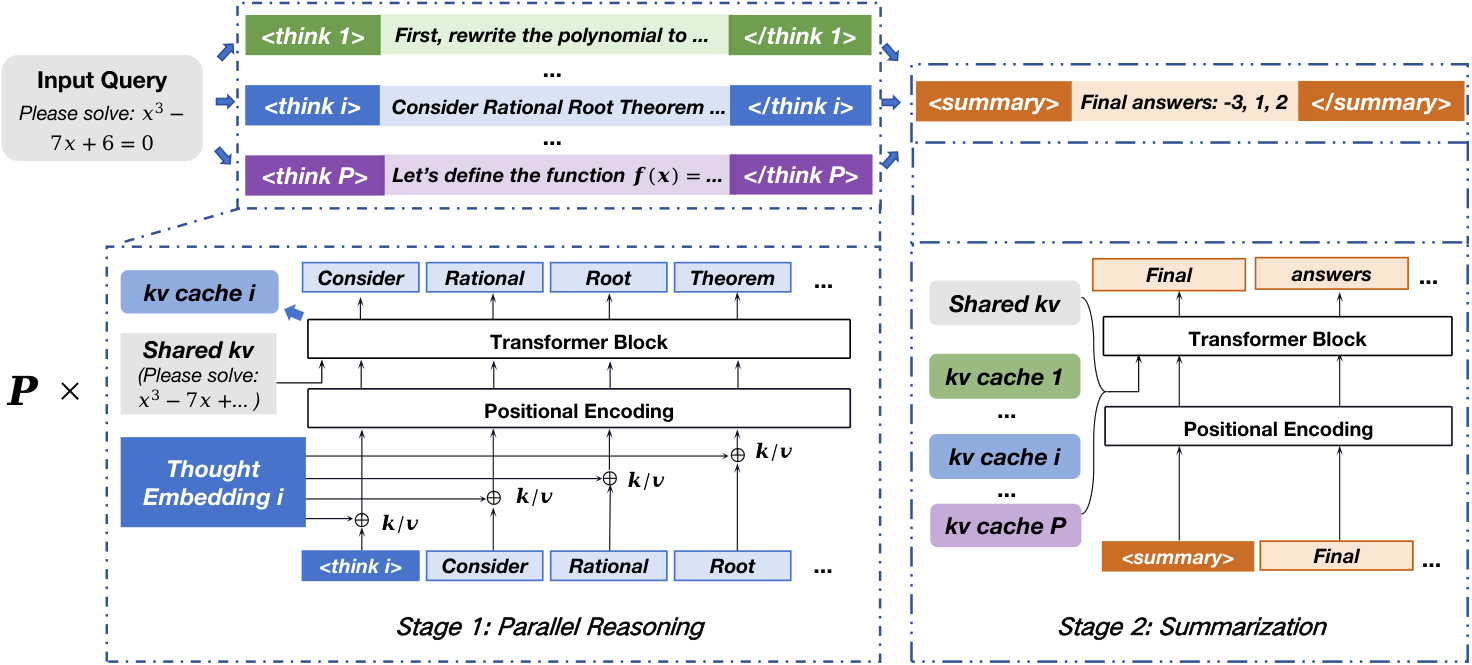
\includegraphics[width=\linewidth,height=0.38\textheight,keepaspectratio]{images/advanced-reasoning/parathinker_main.png}

        \vspace{0.2em}
        \begin{itemize}\itemsep0.3em
            \item \textbf{ParaThinker.} One chain can lock onto an early mistake: ``tunnel vision''. Train the model to think along several paths, isolated by the attention mask, then summarise.
            \item 8 paths: +12.3\% (1.5B) and +7.5\% (7B) over sequential thinking, for 7.1\% more latency.
        \end{itemize}
        \column{0.51\textwidth}
        \begin{itemize}\itemsep0.4em
            \item \textbf{Parallel-R1} teaches the same skill with RL: +8.4\% over sequential RL. Its use of the paths shifts during training from \emph{exploration} to \emph{verification}.
            \item \textbf{Stop early.} DEER watches for a confident trial answer and exits: chains 19 to 80\% shorter, accuracy slightly up.
            \item \textbf{Train it shorter.} Kimi k1.5 rewards short correct answers:
            \[
                \lambda=0.5-\frac{\mathrm{len}-\mathrm{len}_{\min}}{\mathrm{len}_{\max}-\mathrm{len}_{\min}}
            \]
            reward $\lambda$ if correct, $\min(0,\lambda)$ if wrong.
        \end{itemize}
    \end{columns}
    \vspace{0.1em}
    \src{``ParaThinker,'' \href{https://arxiv.org/abs/2509.04475}{arXiv:2509.04475}. ``Parallel-R1,'' \href{https://arxiv.org/abs/2509.07980}{arXiv:2509.07980}. Yang et al., ``Dynamic Early Exit in Reasoning Models,'' \href{https://arxiv.org/abs/2504.15895}{arXiv:2504.15895}. Kimi Team, \href{https://arxiv.org/abs/2501.12599}{arXiv:2501.12599}.}
\end{frame}

\begin{frame}{Neural Search: What to Remember}
    \begin{itemize}\itemsep0.6em
        \item Search can be \textbf{serialised into tokens} and learned. Failed branches are useful training data.
        \item Meta-CoT's claim: reasoning data hides a \textbf{latent search} that models must learn.
        \item RL may mostly \textbf{sharpen} search the base model can already do. The evidence is pass@$k$ at large $k$.
        \item Learned backtracking wins only when the task \textbf{needs depth}.
        \item Efficiency levers: \textbf{compress} the trace, \textbf{parallelise} it, \textbf{stop} it early.
    \end{itemize}
    \vspace{0.3em}
    \vspace{0.2em}
    \takeaway{\textbf{Next.} All the pieces are on the table. How do the actual 2026 reasoning models combine them, and what do their makers disclose?}
\end{frame}
